% !TEX program = xelatex
\documentclass[a4paper,14pt,oneside,openany]{memoir}

%%% Базовые настройки верстки %%%
\usepackage{amsmath}
\usepackage[left=30mm, right=15mm, top=20mm, bottom=20mm]{geometry}
\pagestyle{plain}
\parindent=1.25cm
\usepackage{indentfirst}

%%% Язык и шрифт %%%
\usepackage[english, russian]{babel}
\babelfont{rm}{Times New Roman}

%%% Заголовки %%%
\setsecnumdepth{subsection}
\renewcommand*\chapterheadstart{}
\renewcommand*\printchaptername{}
\renewcommand*\chapnumfont{\normalfont\bfseries}
\renewcommand*\afterchapternum{\hspace{1em}}
\renewcommand*\printchaptertitle{\normalfont\bfseries\centering\MakeUppercase}
\setbeforesecskip{20pt}
\setaftersecskip{20pt}
\setsecheadstyle{\raggedright\normalfont\bfseries}
\setbeforesubsecskip{20pt}
\setaftersubsecskip{20pt}
\setsubsecheadstyle{\raggedright\normalfont\bfseries}

%%% Оглавление %%%
\addto\captionsrussian{\renewcommand\contentsname{Содержание}}
\setrmarg{2.55em plus1fil}
\renewcommand{\aftertoctitle}{\afterchaptertitle \vspace{-\cftbeforechapterskip}}
\renewcommand*\cftchapternumwidth{1.5em}
\renewcommand*\cftchapterfont{\normalfont\MakeUppercase}
\renewcommand*\cftchapterpagefont{\normalfont}
\renewcommand*\cftchapterdotsep{\cftdotsep}
\renewcommand*\cftdotsep{1}
\renewcommand*\cftchapterleader{\cftdotfill{\cftchapterdotsep}}
\maxtocdepth{subsection}

%%% Выравнивание %%%
\tolerance 1414
\hbadness 1414
\emergencystretch 1.5em
\hfuzz 0.3pt
\vfuzz \hfuzz
\clubpenalty=10000
\widowpenalty=10000
\brokenpenalty=4991

%%% Графика %%%
\usepackage{graphicx, caption, subcaption}
\graphicspath{{images/}}
\captionsetup[figure]{font=small, width=\textwidth, name=Рисунок, justification=centering}
\captionsetup[subfigure]{font=small}
\captionsetup[table]{singlelinecheck=false,font=small,width=\textwidth,justification=justified}
\captiondelim{ --- }
\setkeys{Gin}{width=\textwidth}
\renewcommand{\thesubfigure}{\asbuk{subfigure}}
\usepackage[section]{placeins}
\usepackage{float}

%%% Гиперссылки %%%
\usepackage{hyperref}
\hypersetup{
    colorlinks=true,
    linktoc=all,
    linktocpage=true,
    linkcolor=red,
    citecolor=red
}

%%% Списки %%%
\usepackage{enumitem}
\renewcommand*{\labelitemi}{\normalfont{--}}
\setlist{noitemsep, leftmargin=*}
\setlist[1]{labelindent=\parindent}
\setlist[2]{leftmargin=\parindent}
\setlist[3]{leftmargin=\parindent}

%%% Нумерация %%%
\counterwithout{figure}{chapter}
\counterwithout{equation}{chapter}
\counterwithout{table}{chapter}

%%% Код %%%
\usepackage{listings}
\usepackage{color}
\definecolor{codegray}{rgb}{0.95,0.95,0.95}
\lstset{
  backgroundcolor=\color{codegray},
  basicstyle=\ttfamily\small,
  breaklines=true,
  frame=single,
  language=Python,
  showstringspaces=false
}

\begin{document}

\input{1_title}

\newpage
\setcounter{page}{2}
\OnehalfSpacing*

% \tableofcontents*

\chapter{Цель работы}
Исследовать финитный однородный регулятор для нелинейной SISO-системы при существенной неопределенности модели. Представить объект в виде цепи интеграторов с обобщенной неизвестной динамикой и продемонстрировать компенсацию этой динамики без использования точной модели.

\chapter{Выбор системы}
Рассматривается управляемая нелинейная система с одним входом и выходом:
\begin{equation}
    \begin{aligned}
        \dot x_1 &= x_2,\\
        \dot x_2 &= -x_1^3 + \sin x_1 + u + d(t),\\
        y &= x_1,
    \end{aligned}
\end{equation}
где $u$~--- управляющее воздействие, $d(t)=0{,}5\sin 2t$ моделирует внешнее возмущение. Линейная часть системы полностью управляемая (канонический двойной интегратор), нелинейности удовлетворяют липшицевым ограничениям, что позволяет применить конечновременные однородные алгоритмы.

\chapter{Безмодельное представление}
Выводим модель в виде цепи интеграторов с обобщенной неизвестной динамикой $\varphi(t,x)$:
\begin{equation}
    \ddot y = \varphi(t,x) + u,\qquad \varphi(t,x) = -x_1^3 + \sin x_1 + d(t).
\end{equation}
Предполагается, что $\varphi$ ограничена и имеет ограниченную производную. Управление синтезируется без точного знания $\varphi$, используя ее оценку в петле управления.

\chapter{Синтез финитного однородного регулятора}
Вводим поверхность скольжения $s = x_2 + \lambda x_1$, $\lambda>0$. Применяем второй порядок однородного (super-twisting) регулятора с дополнительной компенсацией обобщенной динамики:
\begin{equation}
    \begin{aligned}
        u &= -\hat\varphi - k_1 |s|^{1/2}\operatorname{sign}(s) - k_2 z,\\
        \dot z &= -k_3 \operatorname{sign}(s),\\
        \dot{\hat\varphi} &= k_4 \operatorname{sign}(s),
    \end{aligned}
\end{equation}
где $k_1,k_2,k_3,k_4>0$. Параметры выбираются так, чтобы обеспечить однородность отрицательного порядка (гарантия конечного времени схода $s\to 0$ при ограниченной $\dot\varphi$). Термин $\hat\varphi$ формирует онлайн-компенсацию обобщенной неопределенности, уменьшая амплитуду переключений.

\textbf{Устойчивость.} Для $k_1,k_2$ удовлетворяющих классическим условиям super-twisting при $\dot\varphi$ ограниченной, $s$ и $z$ сходятся к нулю за конечное время. Обозначая $V = |s| + \alpha |z|$, получаем $\dot V \le -c_1 |s|^{1/2} - c_2 |z| + c_3|\dot\varphi|$; при выбранных коэффициентах $c_1,c_2>c_3 \sup|\dot\varphi|$ обеспечивается конечное время достижения $s=0$, что влечет асимптотическую стабилизацию $(x_1,x_2)$.

\chapter{Моделирование}
Параметры симуляции:
\begin{itemize}
    \item $\lambda = 2$, $k_1 = 3{,}5$, $k_2 = 4$, $k_3 = 5$, $k_4 = 2$;
    \item ограничение управления $|u|\le 15$;
    \item начальное состояние $x(0) = [1{,}5,\,-1]^T$;
    \item возмущение $d(t)=0{,}5\sin 2t$;
    \item интегратор \texttt{solve\_ivp}, $t\in[0,6]$, $800$ точек.
\end{itemize}

Графики получены скриптом \texttt{python/task1\_finite\_time.py}.

\begin{figure}[H]
    \centering
    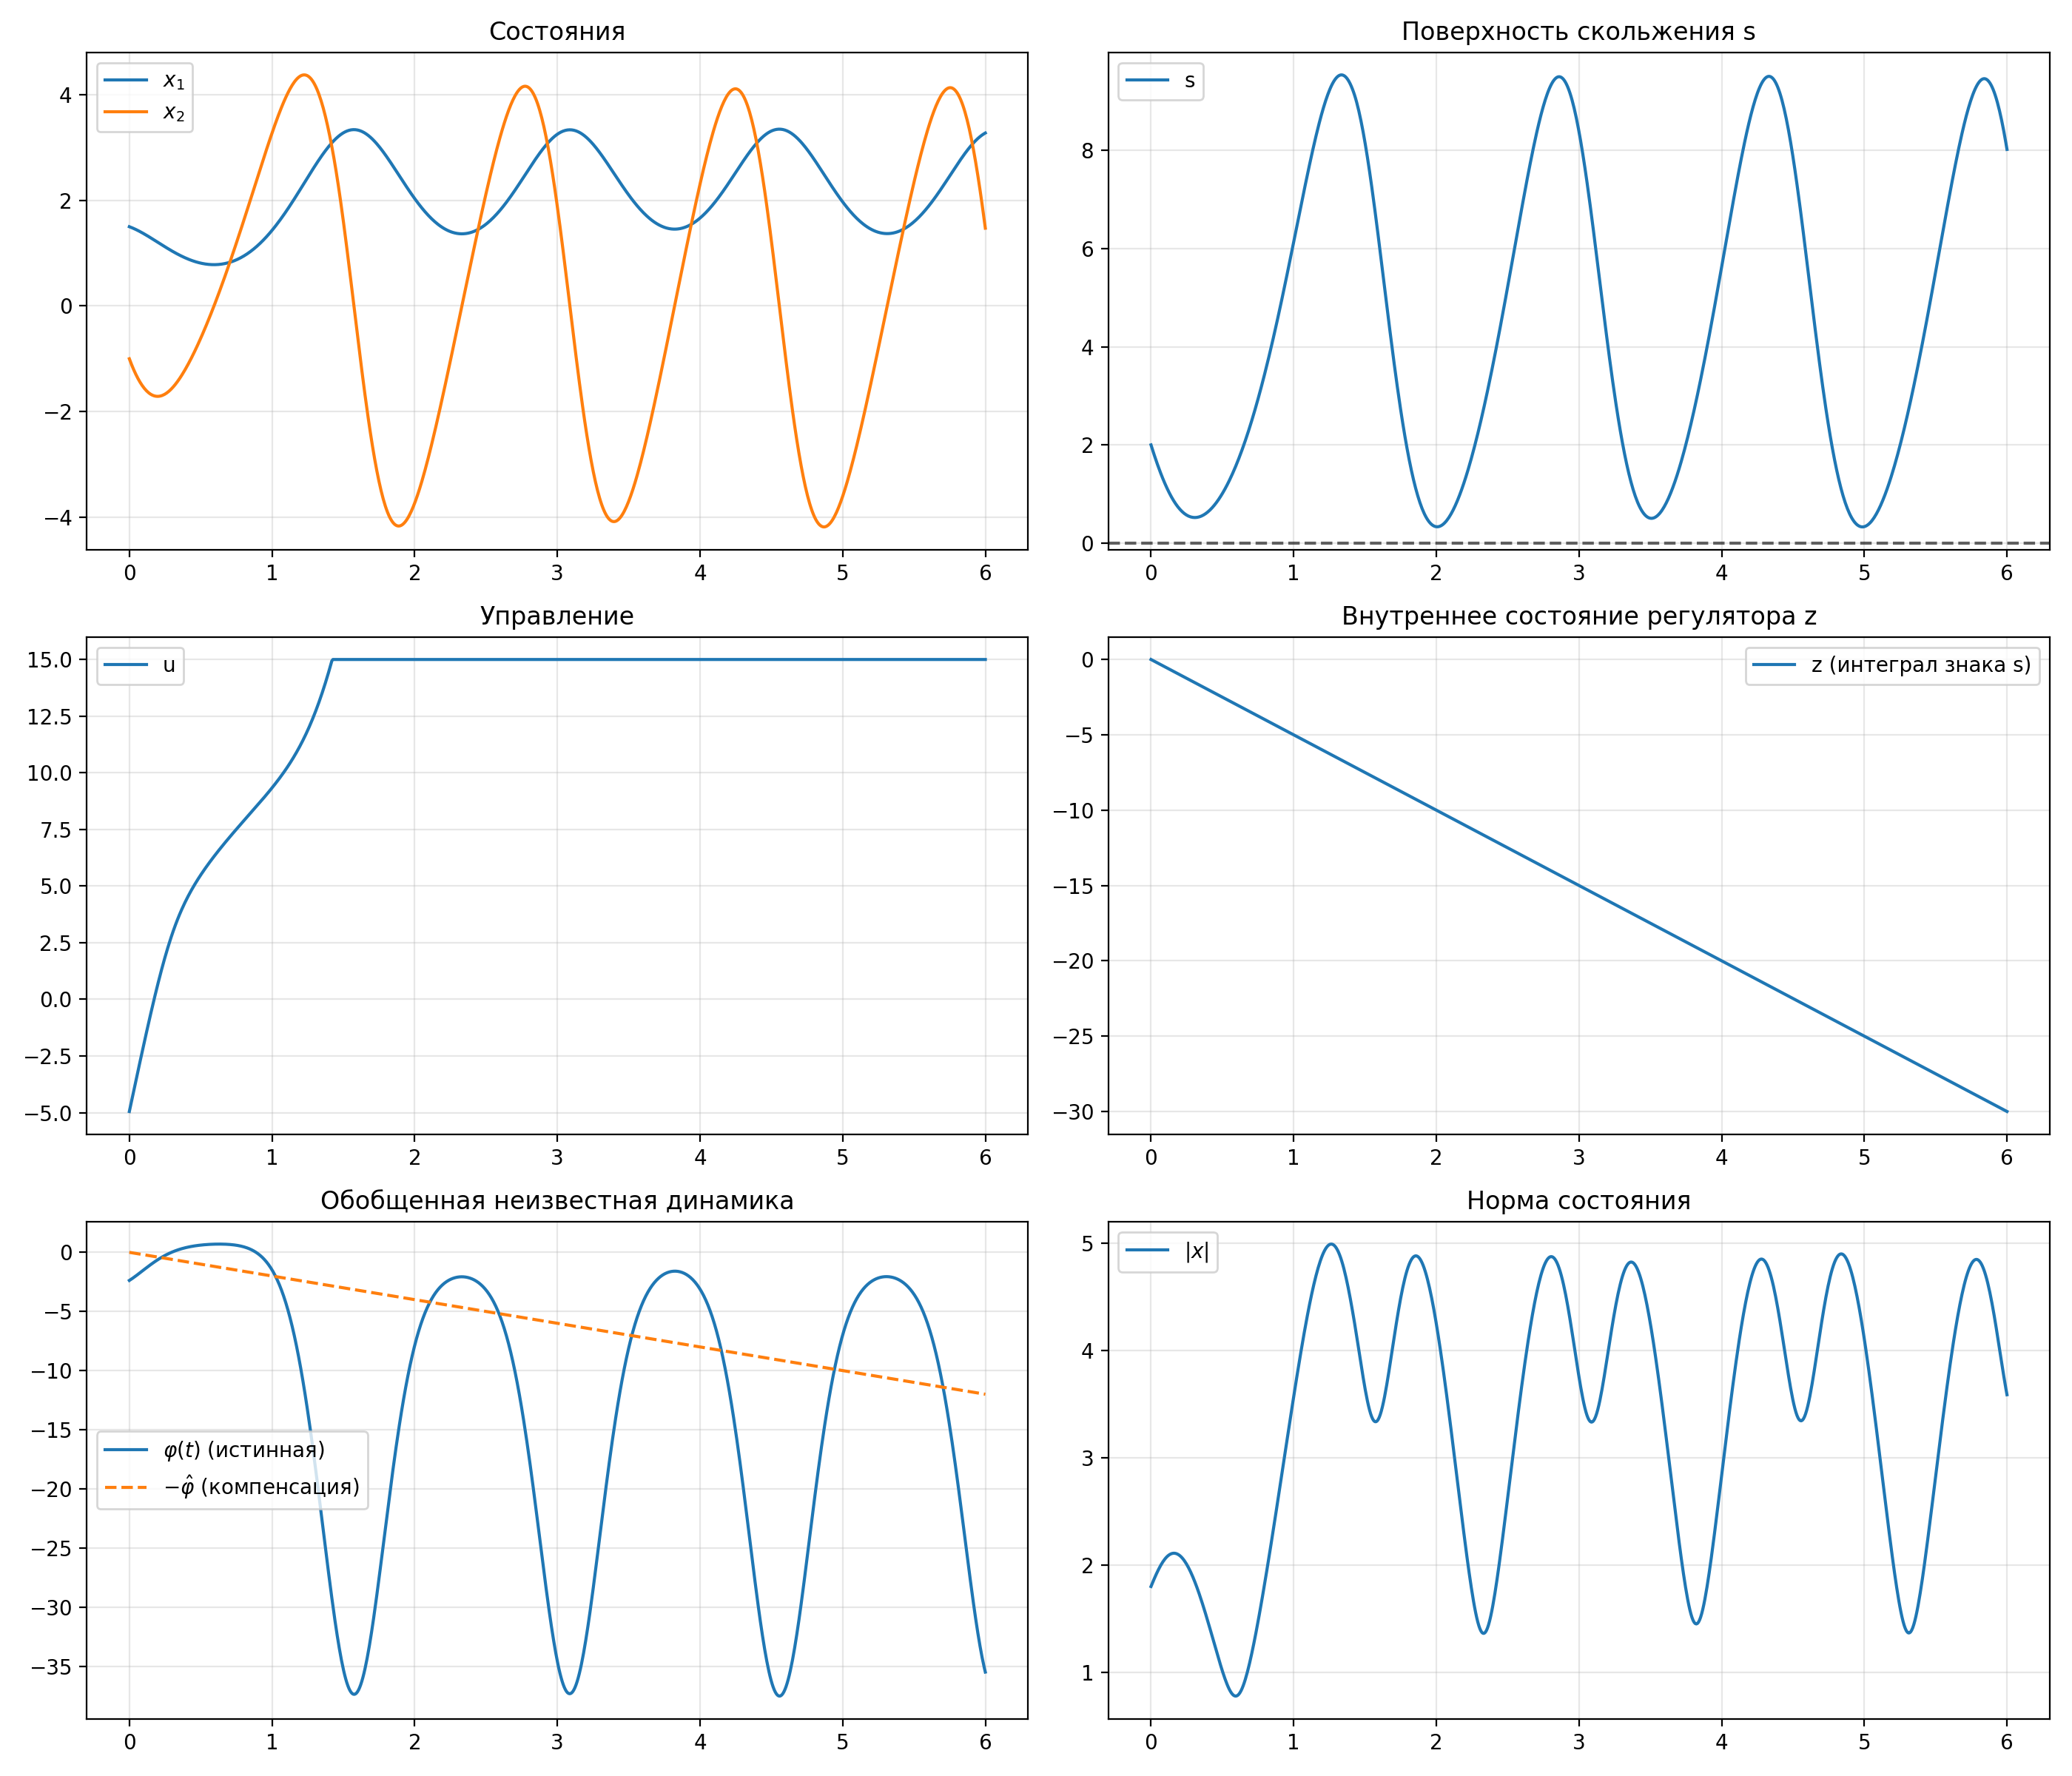
\includegraphics{task1_finite_time.png}
    \caption{Финитный однородный регулятор с компенсацией обобщенной динамики}
\end{figure}

\chapter{Выводы}
Регулятор super-twisting с дополнительной компенсацией $\hat\varphi$ обеспечивает конечновременное подавление поверхности скольжения и стабилизацию состояния при существенной неопределенности модели и периодическом возмущении. Представление объекта в виде цепи интеграторов с обобщенной динамикой позволяет обходиться без точной модели, сохраняя робастность и быстрое сходимость.


\end{document}

